\documentclass[11pt, a4paper]{article}
\usepackage[utf8]{inputenc}
\usepackage{fullpage}
\usepackage{amsmath,amsthm,amsfonts,amssymb,amscd}
\usepackage{subcaption}
\usepackage{lastpage}
\usepackage{enumerate}
\usepackage{fancyhdr}
\usepackage{mathrsfs}
\usepackage{xcolor}
\usepackage{graphicx}
\usepackage{listings}
\usepackage{preamble}
\usepackage{paralist}
\usepackage{ctable}
\usepackage{diagbox}
\usepackage{bm}
\usepackage{geometry}
\usepackage{float}
\usepackage{algorithm}
\usepackage{algorithmic}
\usepackage[colorlinks, linkcolor=blue]{hyperref}
\usepackage{cleveref}
\usepackage{animate}
\geometry{a4paper,scale=0.85}

\definecolor{codegreen}{rgb}{0,0.6,0}
\definecolor{codegray}{rgb}{0.5,0.5,0.5}
\definecolor{codepurple}{rgb}{0.58,0,0.82}
\definecolor{backcolour}{rgb}{0.95,0.95,0.92}

\lstdefinestyle{mystyle}{
    backgroundcolor=\color{backcolour},   
    commentstyle=\color{codegreen},
    keywordstyle=\color{magenta},
    numberstyle=\tiny\color{codegray},
    stringstyle=\color{codepurple},
    basicstyle=\ttfamily\footnotesize,
    breakatwhitespace=false,         
    breaklines=true,                 
    captionpos=b,                    
    keepspaces=true,                 
    numbers=left,                    
    numbersep=3pt,                  
    showspaces=false,                
    showstringspaces=false,
    showtabs=false,                  
    tabsize=2
}

\begin{document}

    \section{Numerical Solution of 2D Heat Equation Using PINN}
    \subsection{Setting Ups}

    We are now investigating numerical solution of the following 2D heat equation:
    \begin{align}
        \begin{cases}
                u_{t}-u_{x x}-u_{y y}=f & x\in (0,1), y\in (0,1), t\in (0,T)\\
                u(0, x, y)=\sin (2 \pi x) \sin (2 \pi y) &\\
                u(t, 0, y)=0 &\\
                u(t, x, 1)=0 &\\
                u_{x}(t, 1, y)=2 \pi e^{-t} \sin (2 \pi y) &\\
                u_{y}(t, x, 0)=2 \pi e^{-t} \sin (2 \pi x) &
        \end{cases}
    \end{align}
    where $f=8\pi^2e^{-t}\sin(2\pi x)\sin(2\pi y)-e^{-t}\sin(2\pi x)\sin(2\pi y)$.
    Its exact solution is $u(t,x,y)=e^{-t}\sin(2\pi x)\sin(2\pi y)$.
    By previous study, we need to generate 5 terms of MSE loss corresponding to the main term, initial condition and boundary conditions. 
    Thus, $u_t$, $u_{xx}$, $u_{yy}$, $u_{x}$, and $u_{y}$ are required to be extracted from the neural network.

    The code snippet of neural network is almost same comparing to the 1D equation.

    Define $f:=u_t-u_{xx}-u_{yy}$, the implementations of $f$, $\text{MSE}_{ic}$, and $\text{MSE}_{bc}$ are listed in code snippet \ref{lst:mse}.

    \lstset{style=mystyle}
    \begin{lstlisting}[language=Python, caption=Implementation of MSEs using PyTorch, label={lst:mse}]
    import torch
    import torch.nn as nn
    from torch import sin, exp
    import numpy as np
    from numpy import pi
s
    from functional import derivative

    def f(model, x_f, y_f, t_f):
        u = model(torch.stack((x_f, y_f, t_f), axis=1))[:, 0]
        u_t = derivative(u, t_f, order=1)
        u_xx = derivative(u, x_f, order=2)
        u_yy = derivative(u, y_f, order=2)
        u_f = ((8*pi**2)-1)*exp(-t_f)*sin(2*pi*x_f)*sin(2*pi*y_f)
        return u_t - u_xx - u_yy - u_f

    def mse_f(model, x_f, y_f, t_f):
        f_u = f(model, x_f, y_f, t_f)
        return (f_u ** 2).mean()

    def mse_0(model, x_ic, y_ic, t_ic):
        u = model(torch.stack((x_ic, y_ic , t_ic), axis=1))[:, 0]
        u_0 = sin(2*pi*x_ic)*sin(2*pi*y_ic)
        return ((u - u_0) ** 2).mean()

    def mse_b(model, x_bc, y_bc, t_bc):
        x_bc_diri = torch.zeros_like(y_bc)
        x_bc_diri.requires_grad = True
        y_bc_diri = torch.ones_like(x_bc)
        y_bc_diri.requires_grad = True
        u_bc_diri = torch.cat((model(torch.stack((x_bc_diri, y_bc, t_bc), axis=1))[:, 0],
                               model(torch.stack((x_bc, y_bc_diri, t_bc), axis=1))[:, 0]))
        mse_dirichlet = (u_bc_diri ** 2).mean()
        x_bc_nuem = torch.ones_like(y_bc)
        x_bc_nuem.requires_grad = True
        y_bc_nuem = torch.zeros_like(x_bc)
        y_bc_nuem.requires_grad = True
        u_bc_nuem_x = model(torch.stack((x_bc_nuem, y_bc, t_bc), axis=1))[:, 0]
        u_bc_nuem_y = model(torch.stack((x_bc, y_bc_nuem, t_bc), axis=1))[:, 0]
        u_x = derivative(u_bc_nuem_x, x_bc_nuem, 1)
        u_y = derivative(u_bc_nuem_y, y_bc_nuem, 1)
        u_x_0 = 2 * pi * exp(-t_bc) * sin(2 * pi * y_bc)
        u_y_0 = 2 * pi * exp(-t_bc) * sin(2 * pi * x_bc)
        mse_neumann = ((u_x - u_x_0) ** 2).mean() + ((u_y - u_y_0) ** 2).mean()
        return mse_dirichlet + mse_neumann
    \end{lstlisting}

    It is worth noting that the generation of collocation and ic\&bc points are using Latin Hypercube Sampling, 
    which was found to require less residual points to achieve the same accuracy as in the case with uniformly placed residual points in PINN. \cite{LHS}
    The implementation of data generation is in code snippet \ref{lst:data}.

    \begin{lstlisting}[language=Python, caption=Implementation of data generation using PyTorch, label={lst:data}]
        def initial_point(size, seed: int = 42):
            set_seed(seed)
            lb = np.array([0.0, 0.0])
            ub = np.array([1.0, 1.0])
            i_f = lb + (ub - lb) * lhs(2, size) # use Latin hypercube sampling
            x_ic = i_f[:, 0]
            y_ic = i_f[:, 1]
            t_ic = np.zeros_like(x_ic)

            return x_ic, y_ic, t_ic

        def bc_point(size, seed: int = 42):
            set_seed(seed)
            lb = np.array([0.0, 0.0, 0.0])
            ub = np.array([1.0, 1.0, 1.0])
            c_f = lb + (ub - lb) * lhs(3, size)
            x_bc = c_f[:, 0]
            y_bc = c_f[:, 1]
            t_bc = c_f[:, 2]
            return x_bc, y_bc, t_bc

        def collocation_point(size, seed: int = 42):
            set_seed(seed)
            lb = np.array([0.0, 0.0, 0.0])
            ub = np.array([1.0, 1.0, 1.0])
            c_f = lb + (ub - lb) * lhs(3, size)
            x_f = c_f[:, 0]
            y_f = c_f[:, 1]
            t_f = c_f[:, 2]
            return x_f, y_f, t_f
    \end{lstlisting}

    When calculating $\bb{L}_2$, evaluating points are evenly aligned (with step size of 0.05) in the region, which do not alter under different hyper-parameters.

    The default hyper parameters are listed in table \ref{table:hp1}.

    \ctable[pos=tbph,
    label=table:hp1,
    mincapwidth = 50mm,
    caption = Settings of hyper parameters.
    ]{c|c}
    {
        \tnote[a]{The learning rate for ADAM.}
        \tnote[b]{The learning rate for L-BFGS.}
    }
    {
        \hline
        Hyper parameter &   value\\
        \hline
        \# Hidden layer  &   6\\
        \# Neurons per layer &   60\\
        \# Initial \& boundary points &   200\\
        \# Collocation points    &   17000\\
        \# epochs    &   200(ADAM)+1200(L-BFGS)\\
        \# Learning rate &   0.005\tmark[a], 1\tmark[b]\\
        Optimization method &   ADAM+LBFGS\\
        Activation function &   Mish\\
        \hline
    }

    \newpage

    \subsection{Mix Method: ADAM + L-BFGS}

    L-BFGS solver is a quasi-Newton method. It estimates the curvature of the searching space via an approximation of the Hessian.
    So it performs well when the neighborhood is relatively flat. 
    L-BFGS may converge slowly or not at all if the starting loss is substantial and the optimization problem is complicated (for instance, in the 2D case).
    L-BFGS incurs additional expenses since every step of the second-order technique requires a rank-two update to the Hessian approximation.
    However, ADAM is a first-order method. The estimate is cruder than that of the L-BFGS in that it is only along each dimension and doesn't account for what would be the off-diagonals in the Hessian.
    Therefore, it is appropriate for the low-accuracy optimization of fluctuating searching space.

    In this 2D heat equation, I compared 6 cases w.r.t. to L-BFGS only, ADAM + L-BFGS with Tanh, GeLU and Mish respectively. The convergence speed and final error are in Figure \ref{fig:al}.
    ADAM optimizer is used for first 200 epochs and L-BFGS takes the rest. Note that using L-BFGS only with Mish, the loss fails to converge.

    \begin{figure}[htb]
        \makebox[\textwidth][c]{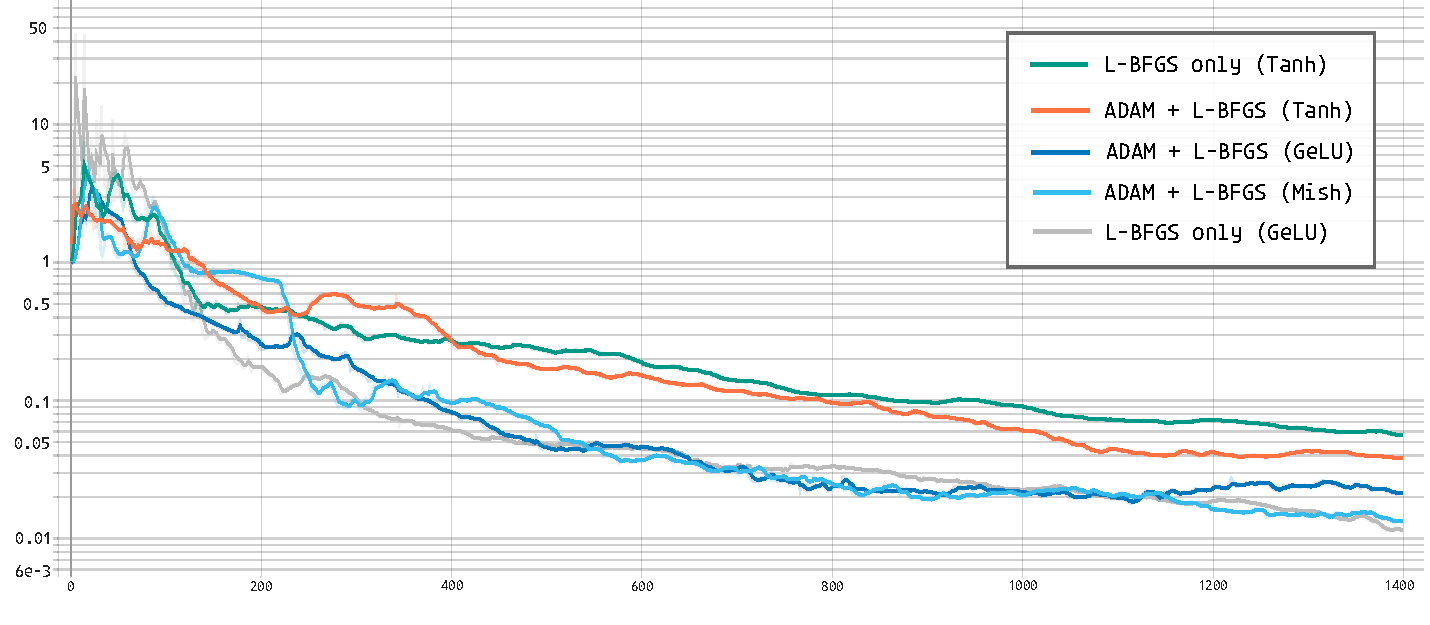
\includegraphics[width=0.9\textwidth]{./pics/MSE_relerror.pdf}}
        \caption{The convergence speed and final error of L-BFGS only and ADAM+L-BFGS. The mix method outperforms using Tanh and Mish but GeLU does not.}
        \label{fig:al}
    \end{figure}

    This mix method outperforms when using Tanh and Mish, but not in GeLU. 
    In fact, in the GeLU scenario, when increase the number of hidden layers, neurons and training points, loss fails to converge. 
    Because the performs for L-BFGS are unstable, it is better used when the loss does not converge or converges very slowly at first, or when the neural network is complicated. 

    \subsection{Getting the result}

    Figure \ref{fig:sol} and \ref{fig:error} show the prediction and error of this equation with hyper-parameters in Table \ref{table:hp1}.
    
    \begin{figure}[htb!]
        \makebox[\textwidth][c]{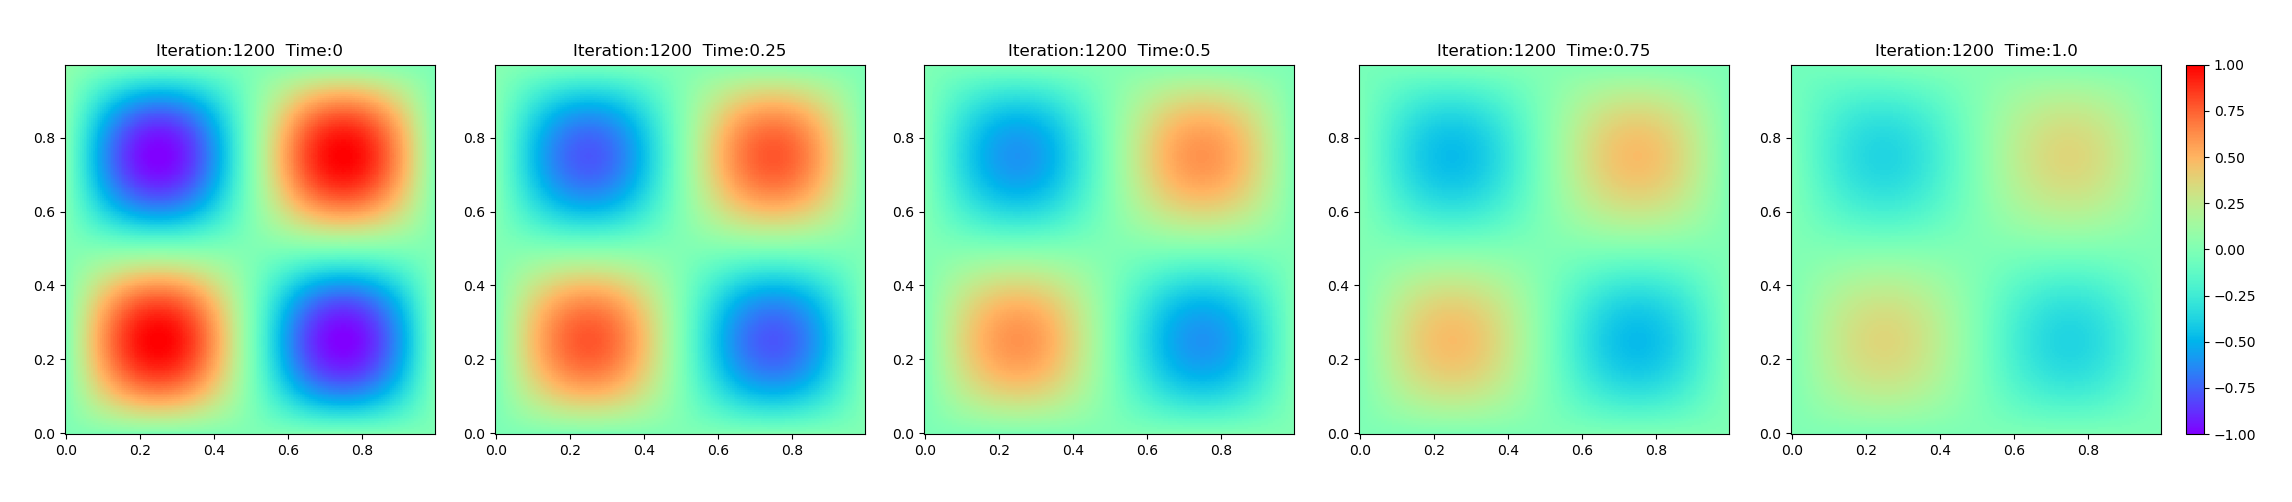
\includegraphics[width=0.9\textwidth]{./pics/sol.png}}
        \caption{The solution at $T=$ 0, 0.25, 0.5, .75 and 1.}
        \label{fig:sol}
    \end{figure}

    \begin{figure}[ht!]
        \makebox[\textwidth][c]{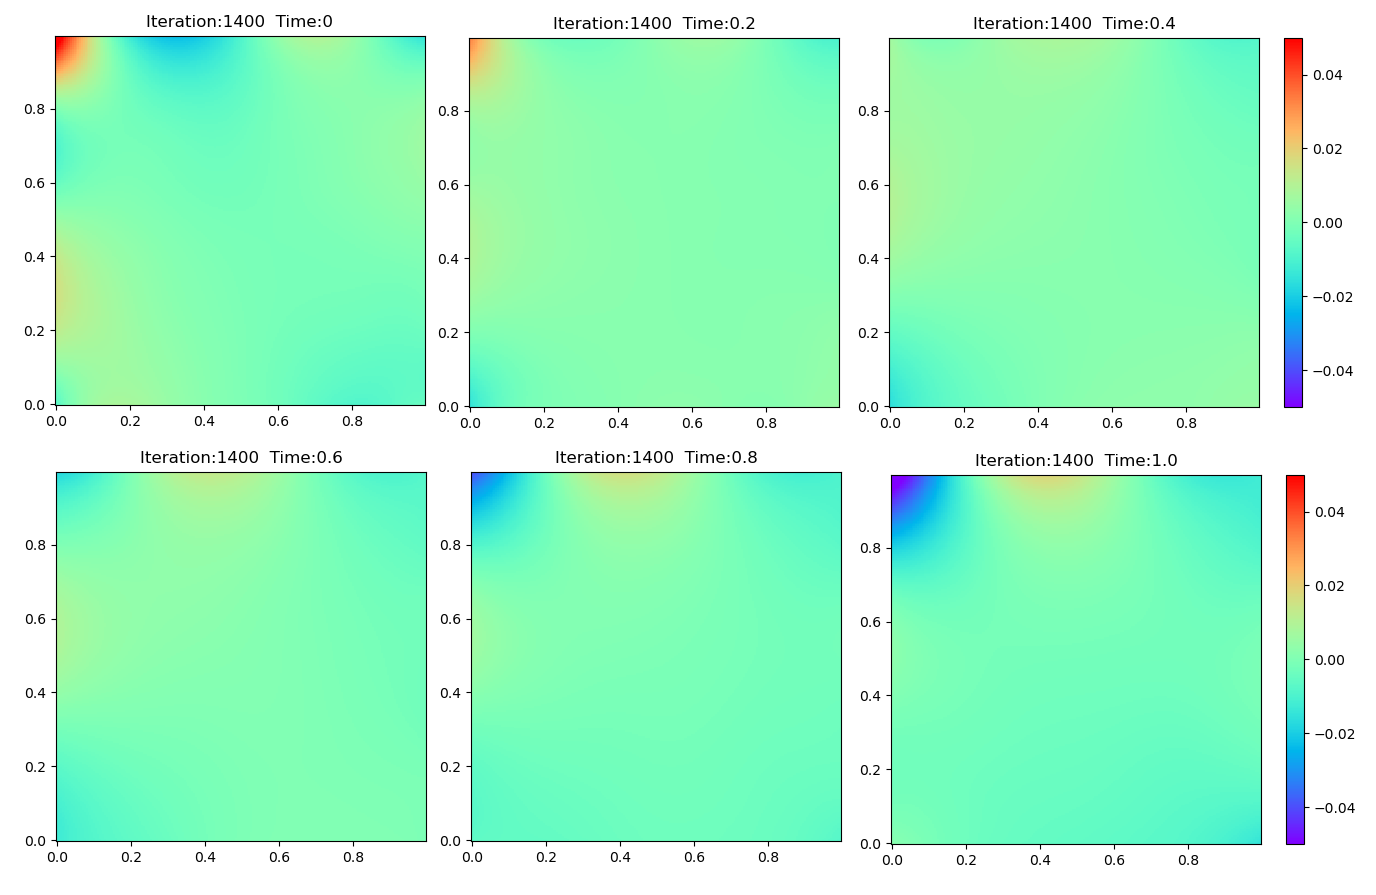
\includegraphics[width=0.9\textwidth]{./pics/error.png}}
        \caption{The error at $T=$ 0, 0.25, 0.5, .75 and 1.}
        \label{fig:error}
    \end{figure}


    Figure \ref{fig:total} shows the points' allocation and the change of relative error from $T=0$ to 1. 

    \begin{figure*}[ht!]
        \centering
          \begin{subfigure}{0.55\textwidth}
            \centering   
            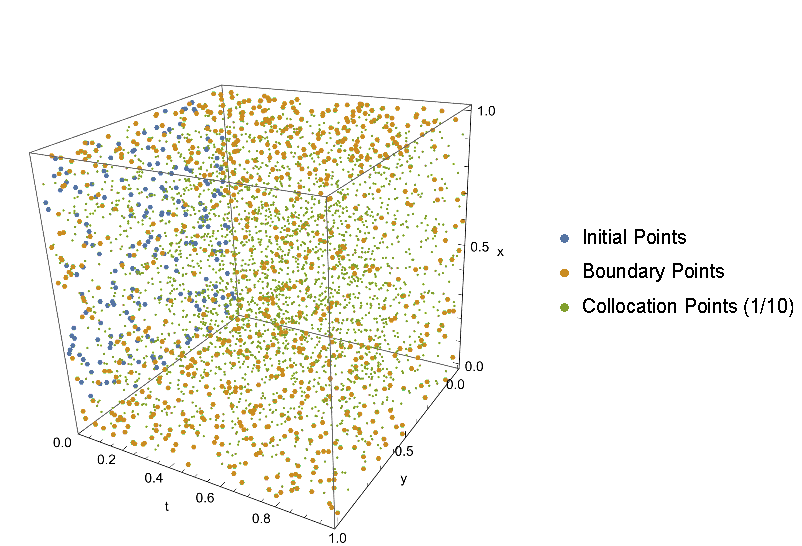
\includegraphics[width=1\linewidth]{./pics/pts.pdf}
              \caption{Points allocation}
              \label{fig:sub1}
          \end{subfigure}   %      \hfill  % 这个\hfill指令为插入弹性长度的空白,看情况选择加不加。
          \begin{subfigure}{0.4\textwidth}
            \centering   
            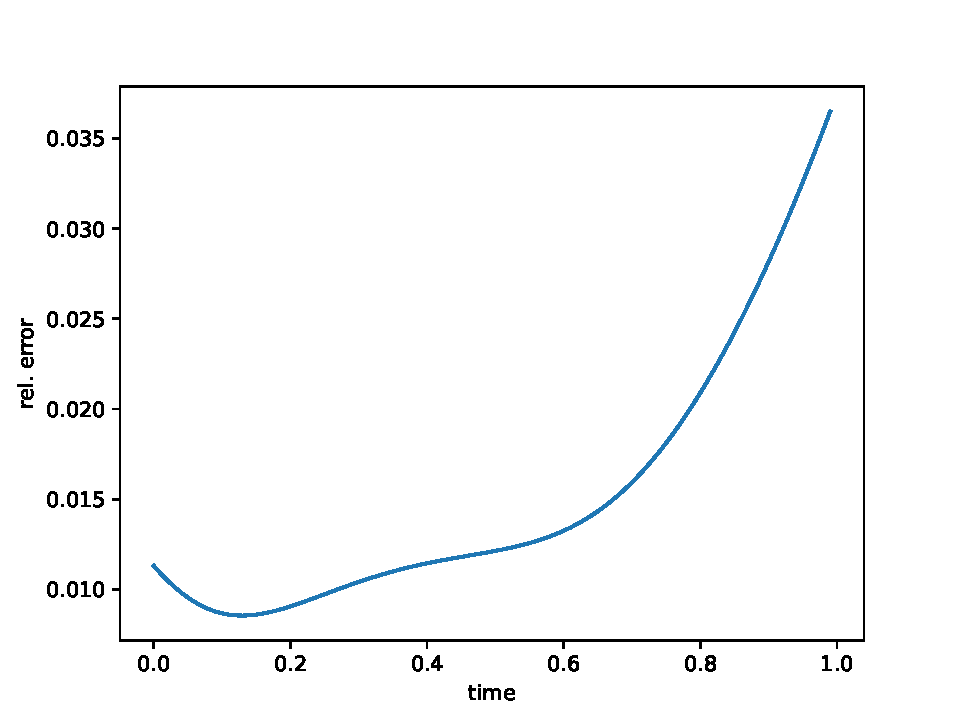
\includegraphics[width=\linewidth]{./pics/rel_error_with_t.pdf}
              \caption{Relative error from $T=0$ to 1}
              \label{fig:relerrorwitht}
          \end{subfigure}
      \caption{
      \label{fig:total}
      Points allocation (Randomly choose 1/ 10 of the col. points) and $\bb{L}_2$ from slices $T=0$ to 1
      }
      \end{figure*}

      Figure \ref{fig:relerrorwitht} reveals that the relative Loss keeps growing with time. This might be because this differential equation has no boundary condition at time T = 1.

    \newpage
    \subsection{Investigation of Hyper-parameters}

    The investigated parameters are listed below:
    \begin{compactenum}
        \item [Network Structure:]~
        \begin{compactenum}
            \item Number of layers: 2, 4, 6, 8, 10
            \item Neurons per layer: 20, 40, 60, 80, 100, 120
        \end{compactenum}
        \item [Optimization:]~
        \begin{compactenum}
            \item Optimization method: L-BFGS, ADAM, ADA, SGD, RMSProp
            \item Activation function: Tanh, GeLU, eLU, Mish, SoftPlus
            \item Epochs (max\_iter for L-BFGS): ADAM(200) + L-BFGS (800, 1000, 1200, 1400, 1600)
            \item Learning rate for L-BFGS: 0.02, 0.1, 1, 2, 5. (Learning rate for ADAM is 0.005)
        \end{compactenum}
        \item[Data:]~
        \begin{compactenum}
            \item Points on initial condition: 50, 100, 150, 200, 250
            \item Points on boundary condition (each boundary): 50, 100, 150, 200, 250
            \item Collocation points: 3000, 10000, 17000, 24000, 24000, 31000, 38000
        \end{compactenum}
    \end{compactenum}
    
    Table \ref{tbl:nn} and \cref{fig:nn} gives the relative error $\bb{L}_2$ between the predicted and 
    the exact solution using different number of hidden layers (2, 4, 6, 8, 10) and neurons per hidden layer (20, 40, 60, 80, 100, 120). 
    Note that the memory consumption is high when use large and deep network.

    \ctable[pos=tbph!,
    mincapwidth = 80mm,
    caption = Relative error (\%) and loss ($10^{-2}$) under different number of hidden layers $N_l$ and neurons per layer $N_n$.,
    label={tbl:nn}
    ]{c|ccccc}
    {
    \tnote[]{$N_i=200$, $N_c=17000$, total epoch=1400 and lr=1, using ADAM + L-BFGS with Mish.}
    \tnote[a]{The result are show in the form \textit{error\ }(\textit{loss})}
    \tnote[b]{The smallest error are in bold font.}
    \tnote[c]{Required VRAM exceeds 16GiB.}
    }
    {
    \hline
    \diagbox{$N_n$}{$N_l$}  & 2     & 4     & 6     & 8     & 10    \\ \hline
     20 & 11.487\ (3.085)\tmark[a] & 4.264\ (1.180)& 2.688\ (0.611)& 4.397\ (1.857)& 5.599\ (1.560)\\
     40 & 2.729\ (0.822)& 2.306\ (0.276)& 2.067\ (0.524)& 4.193\ (0.802)& 3.079\ (0.638)\\
     60 & 2.366\ (0.455)& 1.632\ (0.187)& 1.337\ (0.204)& 1.371\ (0.349)& 1.998\ (0.445)\\
     80 & 2.238\ (0.179)& 1.543\ (\textbf{0.118})\tmark[b] & 1.326\ (0.186)& 1.769\ (0.405)& 3.327\ (0.854)\\
     100 & 1.872\ (0.212)& 2.422\ (0.174)& 1.556\ (0.257)& 2.541\ (0.656)& -\\ 
     120 & 2.396\ (0.270) & 1.455\ (0.153)& \textbf{1.208}\ (0.252) & -\tmark[c] & -\\
     \hline
    }

    \begin{figure}[ht!]
        \makebox[\textwidth][c]{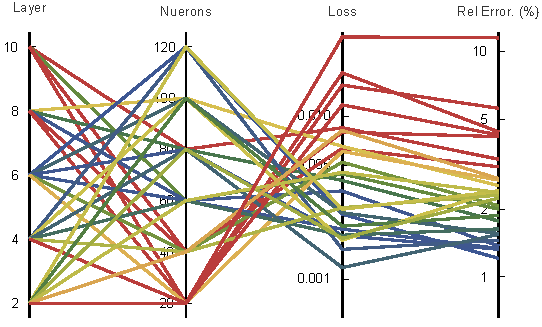
\includegraphics[width=0.7\textwidth]{./pics/pltnn.pdf}}
        \caption{Relative error and loss under different number of hidden layers and neurons per layer.}
        \label{fig:nn}
    \end{figure}

    In general, 6 hidden layers and not less than 60 neurons per layer is the optimal scheme. For the sake of time-saving, $N_n=80$, $N_t=6$ is recommended.


    Table \ref{tbl: data} and \cref{fig:pts} gives the relative error by varying the number of initial and each boundary points (50, 100, 150, 200, 250) and
    collocation points (3000, 10000, 17000, 24000, 24000, 31000, 38000). 

    
    \ctable[pos=th!,
    mincapwidth = 80mm,
    caption = Relative error (\%) and loss ($10^{-3}$) under different number of initial and boundary points $N_i$ and collocation points $N_c$.,
    label= {tbl: data}
    ]{c|ccccc}
    {
    \tnote[]{$N_l=6$, $N_n=60$, total epoch=1400 and lr=1, using ADAM + L-BFGS with Mish.}}
    {
        \hline
        \diagbox{$N_c$}{$N_i$} & 50     & 100     & 150     & 200     & 250     \\ 
        \hline
        3000 & 4.526\ (4.676) & 1.855\ (2.752)	& 2.356\ (2.947) & 4.383\ (6.134) & 1.861\ (3.700)\\
        10000 & 1.425\ (2.338) & 2.028\ (1.989)	& 2.542\ (2.423) & 1.938\ (1.913) & 1.970\ (2.194)\\
        17000 & 1.571\ (2.266) & 2.385\ (2.403)	& 1.488\ (\textbf{1.591}) & \textbf{1.290}\ (1.987) & 1.534\ (1.981)\\
        24000 & 2.721\ (5.077) & 1.782\ (3.067)	& 1.959\ (2.744) & 3.378\ (3.267) & 2.147\ (3.566)\\
        31000 & 2.503\ (1.978) & 1.386\ (1.764)	& 1.642\ (2.260) & 1.932\ (2.110) & 1.681\ (2.203)\\
        38000 & 2.079\ (2.405) & 2.458\ (2.815)	& 3.489\ (3.335) & 1.607\ (2.949) & 1.961\ (2.578)\\
        \hline
    }

    \begin{figure}[ht!]
        \makebox[\textwidth][c]{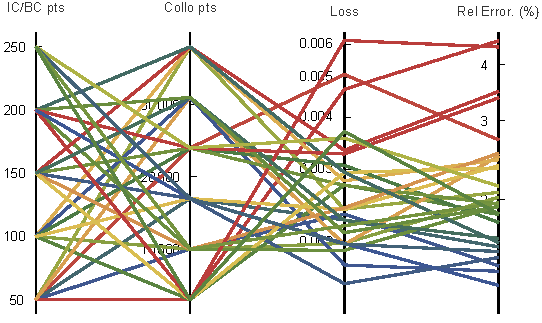
\includegraphics[width=0.7\textwidth]{./pics/pltpts.pdf}}
        \caption{Relative error and loss under different number of initial and boundary points and collocation points.}
        \label{fig:pts}
    \end{figure}

    From the chart and diagram, the number of collocation points is more important than the initial/boundary points. 
    The optimal scheme is found when $N_c=17000$ and $N_i=150$ or $200$ depending on the optimization goal.

    Table \ref{tbl:lr} and \cref{fig:lr} gives the relative error by changing the learning epochs ADAM(200) + L-BFGS (800, 1000, 1200, 1400, 1600) and learning rate for L-BFGS (0.02, 0.1, 1, 2, 5). 

    \ctable[pos=ht!,
    mincapwidth = 100mm,
    caption = Relative error (\%) and loss ($10^{-3}$) under different total epochs $E$ and learning rate.,
    label = {tbl:lr}
    ]{c|cccccc}
    {
    \tnote[]{$N_l=6$, $N_n=60$, $N_i=200$ and $N_c=17000$, using ADAM + LBFGS.}
    }
    {
        \hline
    \diagbox{lr}{$E$} & 1000  & 1200 & 1400 & 1600 & 1800 \\ \hline
    0.02 & 3.174\ (4.685) & 2.217 (4.082) & 1.528\ (2.577) & 1.154\ (2.028) & 0.793 (2.534)\\
    0.1 & 1.394\ (2.691) & 0.827 (2.578) & 0.544\ (1.556) & 0.364\ (1.579) & 0.286 (1.286)\\
    1  & 0.376\ (1.569) & 0.255 (1.503) & 0.186\ (1.326) & 0.136\ (1.261) & \textbf{0.092} (\textbf{1.101})\\
    2  & 0.543\ (1.494) & 0.328 (1.423) & 0.225\ (1.346) & 0.171\ (1.370) & 0.125 (1.183)\\
    6  & 0.593\ (1.622) & 0.380 (1.865) & 0.276\ (1.414) & 0.205\ (1.323) & 0.161 (1.287)\\
    \hline
    }

    \begin{figure}[t!]
        \makebox[\textwidth][c]{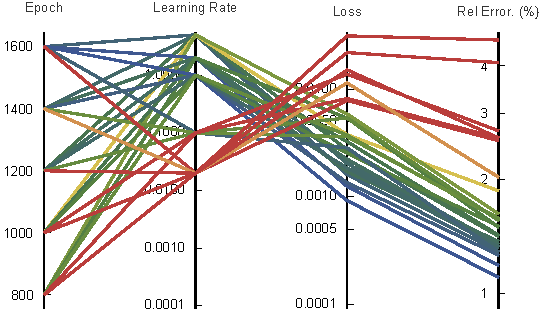
\includegraphics[width=0.7\textwidth]{./pics/pltlr.pdf}}
        \caption{ Relative error and loss under different total epochs and learning rate.}
        \label{fig:lr}
    \end{figure}

    \newpage

    It can be easily seen from \cref{fig:lr} that learning rate of 1 and larger epochs is the optimal scheme here. However, bigger epochs means longer computation elapse. 


    Then, Table \ref{tbl:method} shows the impact of several optimization methods on final loss and error.


    \ctable[pos=!h,
    mincapwidth = 100mm,
    caption = Final loss and error (\%) between the predicted and the exact solution using different optimization methods,
    label = {tbl:method}
    ]{c|ccccc}
    {
    \tnote[]{$N_l=6$, $N_n=60$, $N_i=200$ and $N_c=17000$, total epoch=1400.}}
    {
    \hline
    \diagbox{Attribute}{Opt. Method}  & ADAM + L-BFGS  & ADAM + SGD   & ADA   & RMSProp & ADAM \\ \hline
    Learning Rate & 0.005, 1 & 0.005, 0.00001 & 0.005 & 0.002 & 0.005\\
    ExponentialLR $\gamma$ & - &  0.9995 &  0.9995 & 0.9995 & 0.9995 \\
    Loss  & $\bf{4.676}\tms \bf{10}^{\bf{-3}}$ & 1.310 & 3.695 & 5.865 & 0.058\\
    Rel. Error  & \textbf{1.324} & 74.153 & 70.396 & 36.832 & 7.1634  \\
    \hline
    }

    Finally, as seen in Table \ref{tbl:act}, we get the and final error/loss using various activation functions with default settings. According to the results, Mish still has the fastest convergence and best relative error and  smallest loss comparing to other activation functions. 

    \ctable[pos=!h,
    mincapwidth = 100mm,
    caption = Final loss and error (\%) between the predicted and the exact solution using different activation functions,
    label = {tbl:act}
    ]{c|cccc}
    {
    \tnote[]{$N_l=6$, $N_n=60$, $N_i=200$ and $N_c=17000$, total epoch=1400, using ADAM + L-BFGS.}}
    {
    \hline
    \diagbox{Attribute}{Act. Func.} & Tanh  & GeLU   & Mish   & SoftPlus \\ 
    \hline
    Loss  & $2.380\tms 10^{-3}$ & $1.926\tms 10^{-3}$ & $\bf{1.859}\tms \bf{10}^{\bf{-3}}$ & $7.869\tms 10^{-3}$ \\
    Rel. Error  & 2.215 & 2.560 & \textbf{1.326} & 2.465  \\
    \hline
    }
    
    \newpage

    \subsection{Some notes}

    Using PINN to solve complex partial differential equations may require large sampling and thus consume a lot computation resources (especially VRAM). 
    Numerical solution using traditional numerical method is usually more accurate than PINN but the time consumption need to be compared in the furture if possible. 

    \begin{thebibliography}{9}
        \bibitem{LHS}   Zong, Yifei, QiZhi He, and Alexandre M. Tartakovsky. ``Physics-Informed Neural Network Method for Parabolic Differential Equations with Sharply Perturbed Initial Conditions." arXiv preprint arXiv:2208.08635 (2022).
    \end{thebibliography}

\end{document}